%\part{Aspectos Gerais}

\chapter[Aspectos Gerais]{Aspectos Gerais}

\section{Problemática}

O desenvolvimento da agricultura através de métodos tradicionais vem se mostrando cada dia mais obsoleto, uma vez que não acompanha inovações tecnológicas.(FALTA REF.) Essa transferência de tecnologia para aplicações práticas em processos produtivos muitas vezes ocorre de forma lenta, já que os produtores se mostram resistentes a alterações em um sistema que funciona relativamente bem. Entretanto, a não adoção dessas tecnologias acarreta prejuízos das mais diversas formas. Ao abdicar de uma análise detalhada do solo, um produtor agrícola gera custos desnecessários de irrigação, nutrição do solo, controle de acidez, além da inevitável queda na qualidade do produto final. Mesmo que exista uma análise laboratorial por amostragem, esse método não demonstra ser tão eficiente quanto uma análise automatizada, já que essa análise somente é feita em laboratórios específicos, podendo a amostra, durante o seu transporte, ter alterações em suas características, o que pode prejudicar o resultado final da análise. Uma produção baseada em inovações tecnológicas garante, portanto, o aumento de produtividade, diminuição de custos e reduz significativamente possíveis falhas humanas no diagnóstico de problemas.

\begin{comment}
\begin{description}
	\item [Pré-textuais] \

	\begin{itemize}
		\item Capa
		\item Folha de rosto
		\item \textit{Dedicatória}
		\item \textit{Agradecimentos}
		\item \textit{Epígrafe}
		\item Resumo
		\item Abstract
		\item Lista de figuras
		\item Lista de tabelas
		\item Lista de símbolos e
		\item Sumário
	\end{itemize}

	\item [Textuais] \

	\begin{itemize}
		\item \textbf{\textit{Introdução}}
		\item \textbf{\textit{Desenvolvimento}}
		\item \textbf{\textit{Conclusões}}
	\end{itemize}

	\item [Pós-Textuais] \
	
	\begin{itemize}
		\item Referências bibliográficas
		\item \textit{Bibliografia}
		\item Anexos
		\item Contracapa
	\end{itemize}
\end{description}

Os aspectos específicos da formatação de cada uma dessas três partes 
principais do relatório são tratados nos capítulos e seções seguintes.

No modelo \LaTeX, os arquivos correspondentes a estas estruturas que devem
ser editados manualmente estão na pasta \textbf{editáveis}. Os arquivos
da pasta \textbf{fixos} tratam os elementos que não necessitam de 
edição direta, e devem ser deixados como estão na grande maioria dos casos.
\end{comment}

\section{Estado da Arte}

Dentre as tecnologias existentes, protótipos como o rover, desenvolvido pela Embrapa em conjunto com a Universidade de São Paulo, e o “Robô Autônomo para Monitoramento do Solo” pela Universidade de Virgínia, se destacam como potenciais tecnologias no ramo da automatização agrícola e possuem grande potencial de inserção no mercado.  Entretanto estas tecnologias não são amplamente utilizadas no mercado por se tratarem de protótipos e não haver produção em massa consolidada.

O rover desenvolvido pela EMBRAPA utiliza uma tecnologia de análise óptica para adquirir dados do solo. Essa tecnlogia se chama LIBS (Espectroscopia de emissão óptica com plasma induzido por laser), onde um laser de alta energia é focalizado sobre o solo, fazendo com que seja formado um plasma. Esse plasma realiza uma análise multielementar do solo. (ARCHILA, 2014).

\clearpage

\begin{figure}[!htb]
	\centering
	\label{figura1}
	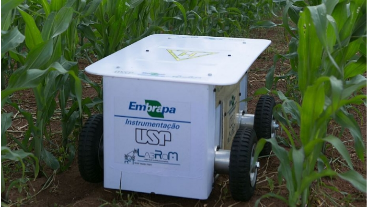
\includegraphics[scale=0.6]{figuras/figura1}
	\caption{Rover da EMBRAPA com tecnlogia LIBS. Fonte: ARCHILA, 2014.}
\end{figure}

Esse rover utiliza dois motores de corrente direta (DC) BTS7960 Arduino, três baterias de 12 Volts e 7 Ampére-hora, um conversor 3,3-5 Volts, e a arquitetura é formada por um microcontrolador Raspberry-pi, encarregado de enviar sinais de controle para o sistema de propulsão, além de ter os motores ligados a um Arduino UNO, encarregado de gerar sinais de PWM (Pulse-width modulation), controlando assim o sentido de giro dos motores e suas velocidades (ARGOTE, 2014).

\section{Justificativa}

A produção agropecuária no Brasil não está em dia com a sustentabilidade. O setor que mais consome é também o que mais desperdiça água doce no país. Aproximadamente 70\% da água é destinada as suas atividades e quase metade desse valor é jogada fora. Entre os motivos do desperdício estão irrigações mal executadas e falta de controle do agricultor na quantidade usada em lavouras e no processamento dos produtos (FAO 2013).

Além do desperdício, a má administração do recurso hídrico tem impacto direto na produtividade. A umidade do solo pode representar a diferença entre o sucesso e o fracasso de uma lavoura, principalmente para o plantio de espécies sensíveis a variações climáticas, como o morango, que exige um alto controle desse fator, em níveis acerca de 75\% (Referencia).

Desta forma, é clara a necessidade de um sistema que seja capaz de monitorar a umidade do solo, tornando possível melhorar as condições do plantio e consequentemente aumentar os níveis de produtividade, reduzindo custos com perdas e desperdícios e dando mais qualidade ao produto final.

\subsection{Viabilidade Técnica e Financeira}

A fazer

%da página evitando-se a \lq\lq quebra\rq\rq\ da figura ou tabela. 

\section{Escopo}

A fazer

\section{Objetivo}

\subsection{Geral}

O projeto possui como objetivo construir um veículo terrestre autônomo que possa aferir os valores de umidade do solo, ar e temperatura em uma plantação de morangos para que seja realizado um controle adequado em tais parâmetros.

\subsection{Específico}

\begin{itemize}	
	\item Analisar componentes do veículo;
	\item Identificar meio de locomoção para o ambiente;
	\item Escolher técnica de medição adequada para as variáveis impactantes (umidade do solo e ar e temperatura do ar);
	\item Desenvolver sistema de localização para autonomia do veículo;
	\item Criar uma plataforma para a apresentação dos dados coletados.
\end{itemize}
